\documentclass[aspectratio=169]{beamer}
\usetheme{Copenhagen}
\usecolortheme{whale}
\usefonttheme[onlymath]{serif}
\addtobeamertemplate{footnote}{\hskip -2em}{}

\usepackage{setspace}
\usepackage{xcolor}
\usepackage{graphicx}
\usepackage{multimedia}
\usepackage{fontawesome5}
\usepackage[most]{tcolorbox}
\usepackage{empheq}
\usepackage{fancybox}
\usepackage{annotate-equations}
\usepackage{soul}
\usepackage{tikz}
\usetikzlibrary{positioning, calc, shapes.geometric, shapes.multipart, 
	shapes, arrows.meta, arrows, 
	decorations.markings, external, trees}
\tikzstyle{Arrow} = [
thick, 
decoration={
	markings,
	mark=at position 1 with {
		\arrow[thick]{latex}
	}
}, 
shorten >= 3pt, preaction = {decorate}
]

\definecolor{teel}{HTML}{00AEB3}
\definecolor{redorange}{HTML}{F26035}
\definecolor{darkred}{HTML}{8B0000}
\definecolor{darkblue}{HTML}{00008B}
\definecolor{darkgreen}{HTML}{06402B}
\definecolor{CarolinaBlue}{HTML}{4B9CD3}
\definecolor{deepsea}{HTML}{123456}
\definecolor{sharedblue}{HTML}{009292}
\definecolor{distalblue}{HTML}{490092}

\usecolortheme[named=CarolinaBlue]{structure}

\title[Positivity Violations]{Sensitivity analyses for positivity violations}
\author[PN Zivich]{Paul Zivich \\ Assistant Professor \\ Department of Epidemiology \\ University of North Carolina at Chapel Hill}
\date{June 24, 2026}

\setbeamercovered{transparent}
\setbeamertemplate{navigation symbols}{}  % gets rid of the dumb navigation symbols
\setbeamertemplate{page number in head/foot}{\insertframenumber}  % adds slide #
\setbeamertemplate{headline}{}

\newcommand\blfootnote[1]{%
	\begingroup
	\renewcommand\thefootnote{}\footnote[frame]{#1}%
	\addtocounter{footnote}{-1}%
	\endgroup
}

\AtBeginSection[]{
	\begin{frame}
		\vfill
		\centering
		\begin{beamercolorbox}[sep=8pt,center,shadow=true,rounded=true]{title}
			\usebeamerfont{title}\insertsectionhead\par%
		\end{beamercolorbox}
		\vfill
	\end{frame}
}

\begin{document}
	
\begin{frame}[plain]
	\maketitle
\end{frame}

\begin{frame}{Acknowledgments\footnote[frame]{Footnotes are for asides or references}}
	\textbf{Funding}: K01AI177102
	~\\~\\
	\textbf{Conflicts of Interest}: None
	~\\~\\
	\textbf{Acknowledgments}: Stephen Cole, Jess Edwards, Bonnie Shook-Sa, Eric Lofgren
	~\\~\\
	\textbf{Disclaimer}: All errors are my own
	~\\~\\
	\textbf{Publication}: Zivich et al. \textit{J Epidemiol Community Health} 2026;80:352-356
	~\\~\\
	\begin{center}
		\small
		\faEnvelope \quad pzivich@unc.edu \qquad \quad 
		\faGithub \quad pzivich \qquad \quad
		\faHashtag \quad pausalz@bsky.social
	\end{center}	
\end{frame}

\begin{frame}{Motivating Example}
	\textbf{Question}: What is the mean systolic blood pressure (SBP) in mm Hg among children and adolescents aged 2-17 in the United States?
	\\~\\~\\
	\textbf{Parameter}: $\mu = E[Y]$ where $Y_i$ is SBP, and $E[\cdot]$ is the expected value function\footnote[frame]{Can think about $E[\cdot]$ as $1/n \sum_{i=1}^{n} (\cdot)$}
	~\\~\\~\\
	\textbf{Data}: NHANES 2017-2018
	~\\~\\~\\
	\textbf{Systematic Error}: SBP is missing for 44\% of children	
\end{frame}

\begin{frame}{Missing Data}
	Extent of missingness means that estimate is sensitive to choices about missing data
	~\\~\\~\\
	For example, a complete-case analysis assumes
	$$ E[Y] = E[Y \mid R=1] $$
	where $R_i$ denotes an indicator of SBP being measured
\end{frame}

\begin{frame}{A Weaker Assumption}
	Instead of a complete-case analysis, we can assume that SBP is missing completely at random conditional on $X$ (i.e., conditionally exchangeable)
	\begin{equation*}
		E[Y \mid X=x] = E[Y \mid X=x, \eqnmarkbox[gray]{node0}{R=1}] \text{ for all values of } x
	\end{equation*}
	\annotate[yshift=-0.2em]{below,left}{node0}{Can freely condition on}	
	~\\
	Under this assumption, $\mu$ is identified by\footnote[frame]{Estimate with direct maximum likelihood estimator, g-computation}
	\begin{equation*}
		\sum_{x \in \mathcal{X}} E(Y \mid X=x, R=1) \Pr(X=x)
	\end{equation*}
	or a weighted average of the complete-case means within strata of $X$
\end{frame}



\begin{frame}{Positivity}
	Exchangeability necessitates a \textit{positivity} assumption
	~\\~\\
	\textbf{Definition}:
	~\\~\\
	\begin{equation*}
		\eqnmarkbox[deepsea]{node1}{\Pr(R=1 \mid X=x)} \eqnmarkbox[redorange]{node2}{> 0} 
		\eqnmarkbox[distalblue]{node3}{\forall x \in \mathcal{X}}
	\end{equation*}
	\annotate[yshift=0.5em]{above,left}{node1}{Probability of $Y$ being observed}	
	\annotate[yshift=0.5em]{above,right}{node2}{is non-zero}	
	\annotate[yshift=-0.2em]{below,left}{node3}{for all unique values of $X$}	
	~\\~\\~\\
	Intuitively, we need some individuals with $X=x$ to have $Y$ observed at least sometimes so can `stand-in' for those without $Y$ measured
\end{frame}

\begin{frame}{Positivity for SBP in NHANES}
	If $X$ is age, then positivity can be depicted as \\~\\
	\begin{center}
		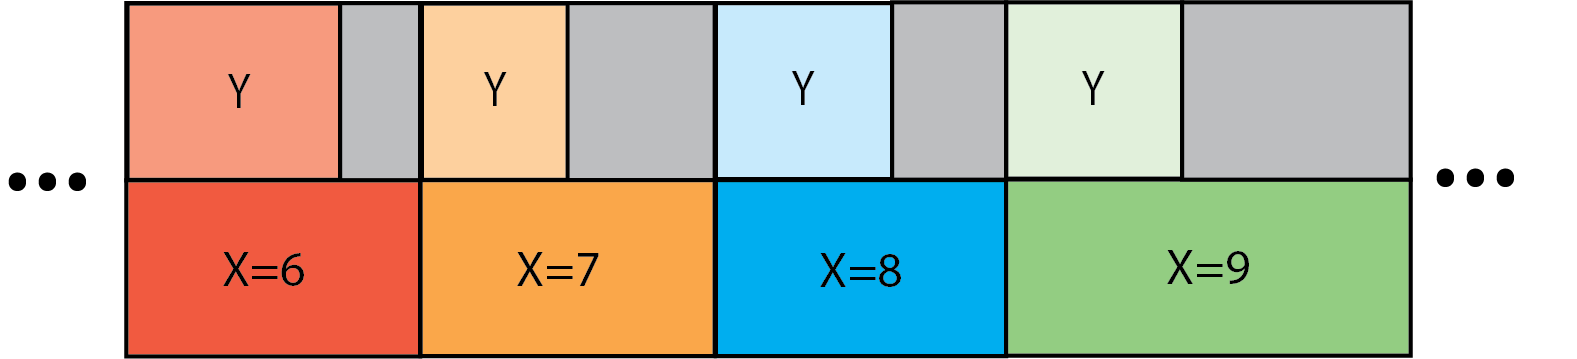
\includegraphics[width=0.85\linewidth]{images/missing-diagram1.png}
	\end{center}
	~\\
	Every unique age in the population has some individuals with SBP measured
\end{frame}

\begin{frame}{Nonpositivity by Age in NHANES}
	In NHANES 2017-2018,
	\begin{itemize}
		\item ``BP is measured on participants 8 years and older"\footnote[frame]{\url{https://wwwn.cdc.gov/Nchs/Nhanes/2017-2018/BPX_J.htm}}
	\end{itemize}
	~\\
	\begin{center}
		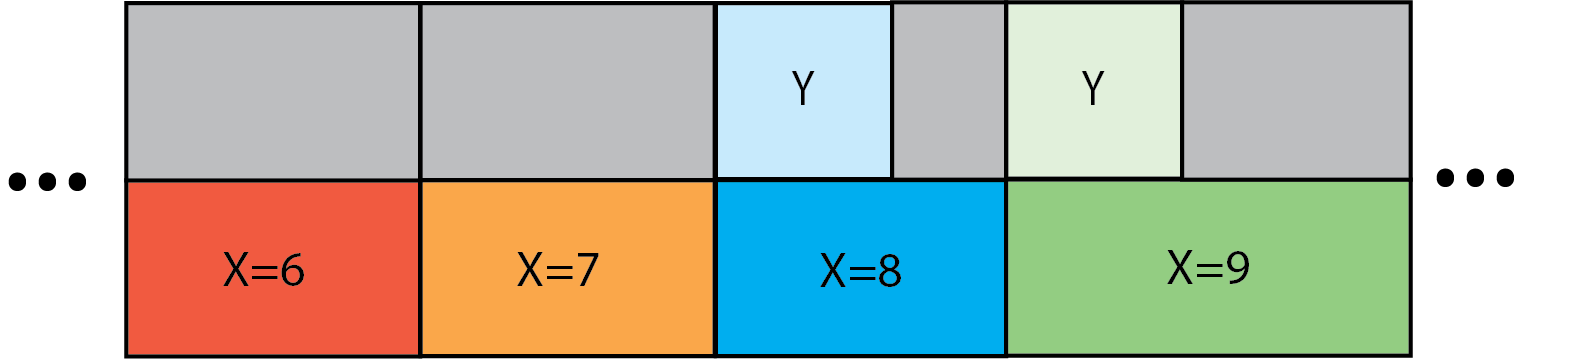
\includegraphics[width=0.85\linewidth]{images/missing-diagram2.png}
	\end{center}	
\end{frame}

\begin{frame}{NHANES Data}
	\begin{center}
		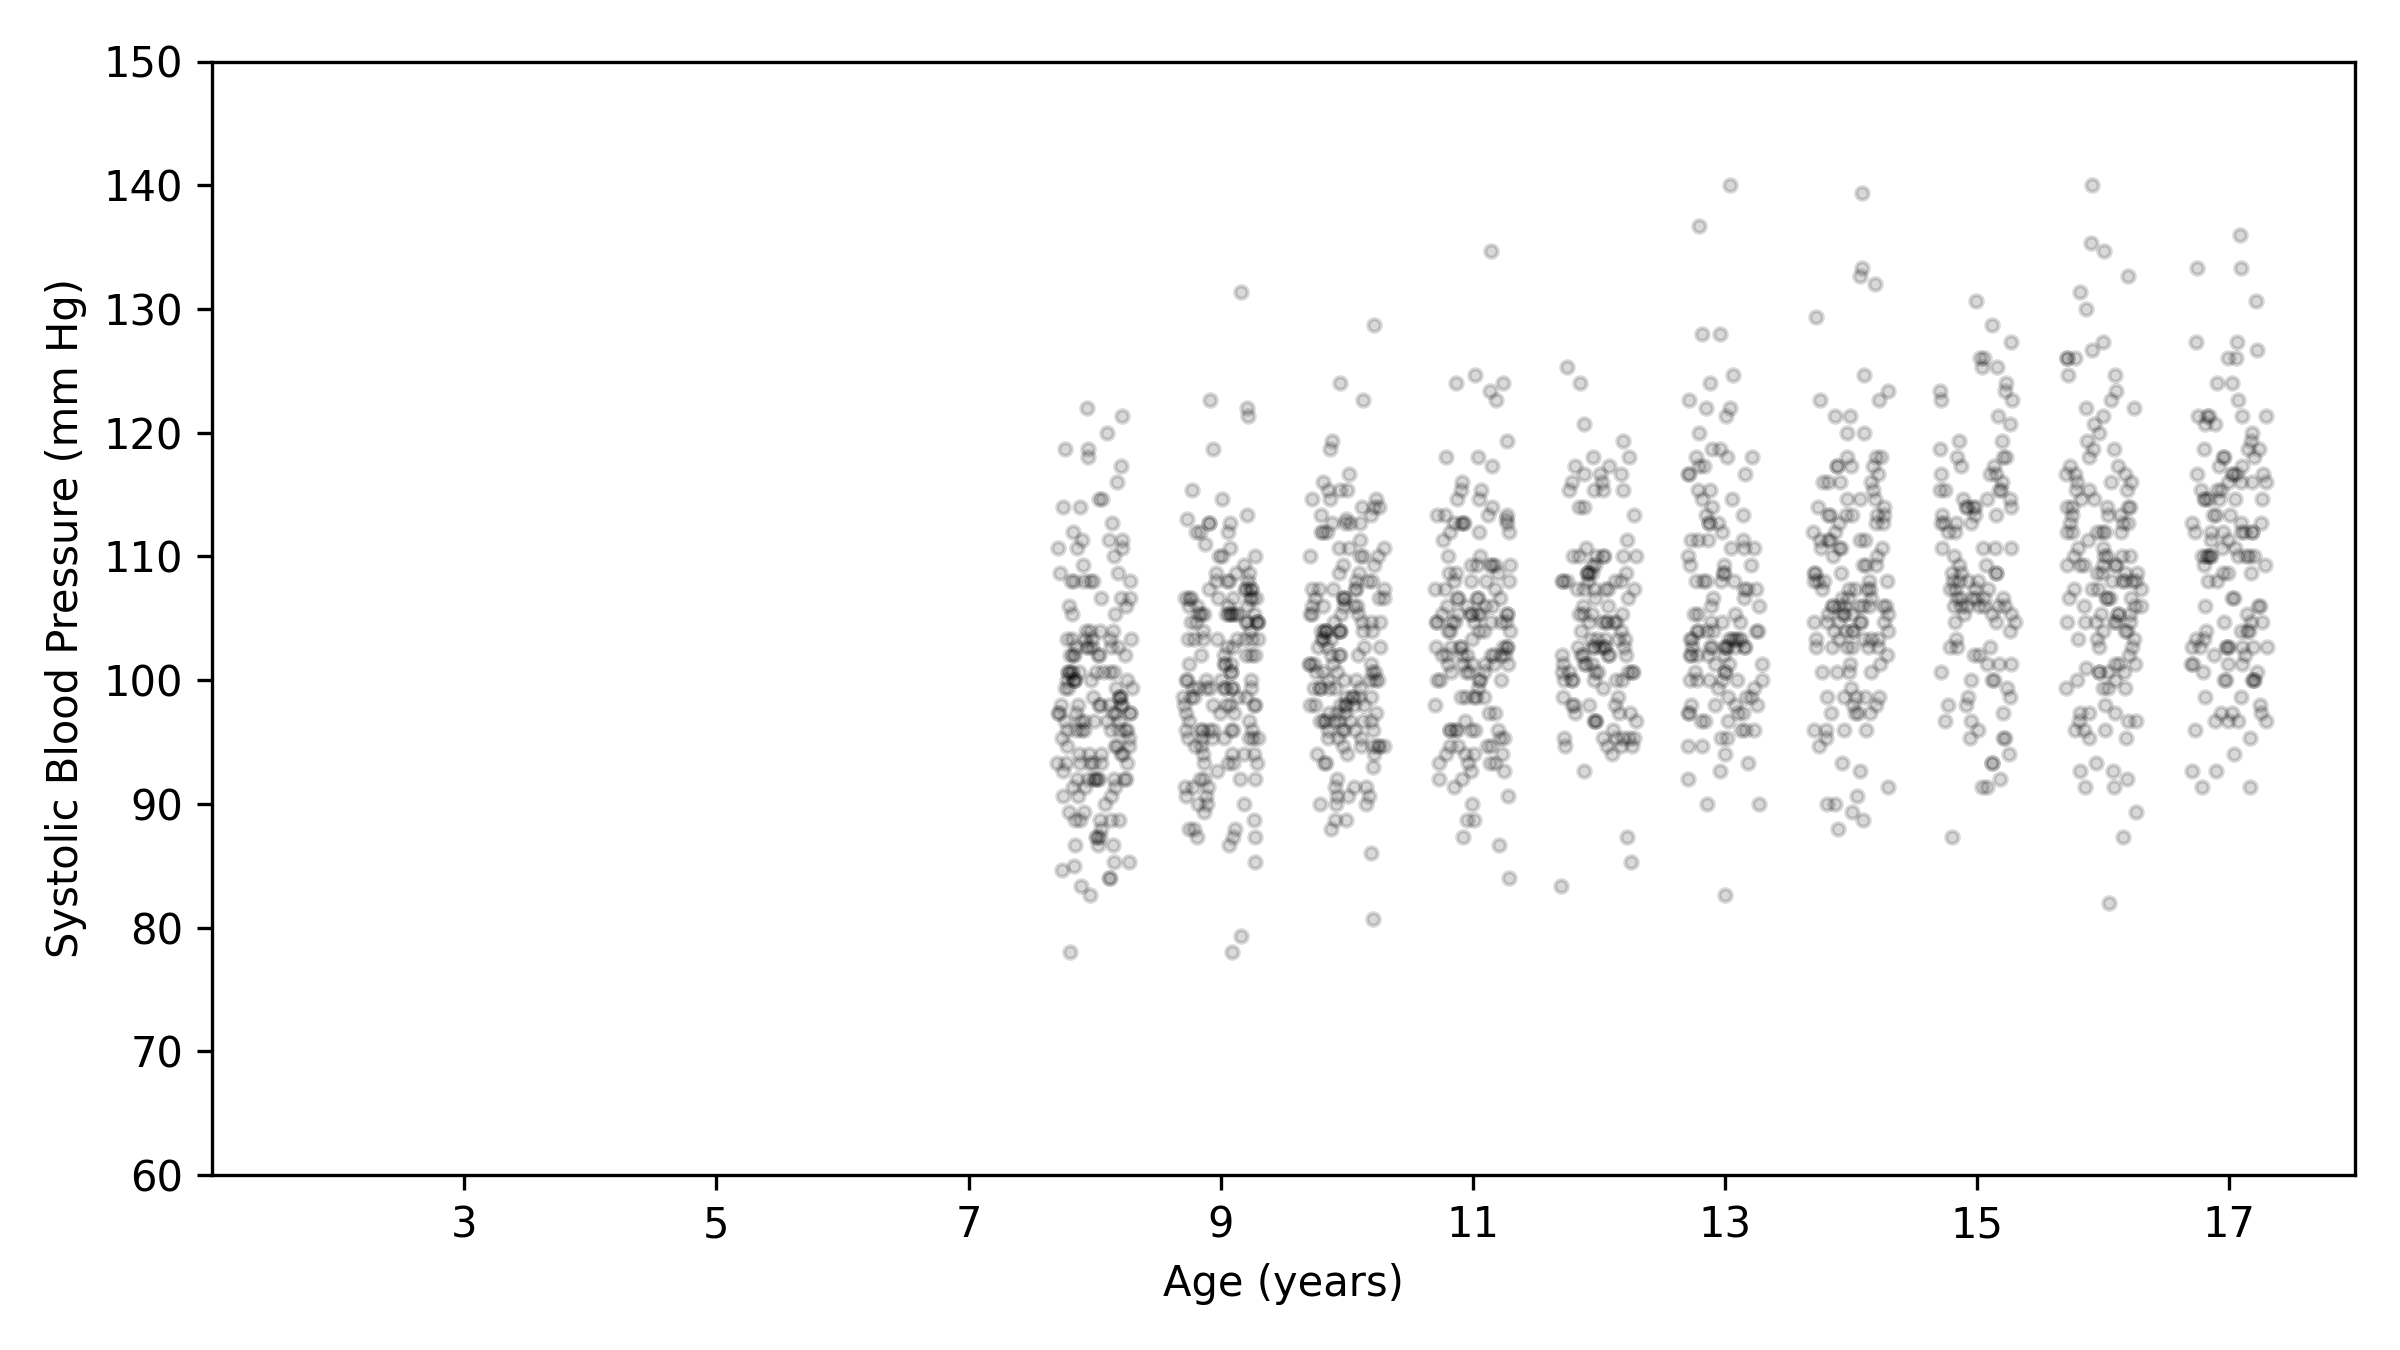
\includegraphics[width=0.92\linewidth]{images/missing_nhanes1.png}
	\end{center}
\end{frame}

\begin{frame}{Addressing Positivity Violations}
	Consider two routine methods for dealing with positivity violations
	\begin{itemize}
		\item[1.] Change the parameter
		\item[2.] Extrapolate from a model 
	\end{itemize}
\end{frame}

\begin{frame}{Option 1: Change the Parameter}
	\textbf{Parameter (revised)}: mean SBP {\color{darkred} for those 8 or older}
	$$ \mu^* = E[Y \mid X \ge 8] $$
	\textbf{Question}: what is the mean systolic blood pressure (SBP) in mm Hg among children and adolescents {\color{darkred} aged 8-17} in the US?
	~\\
	\begin{center}
		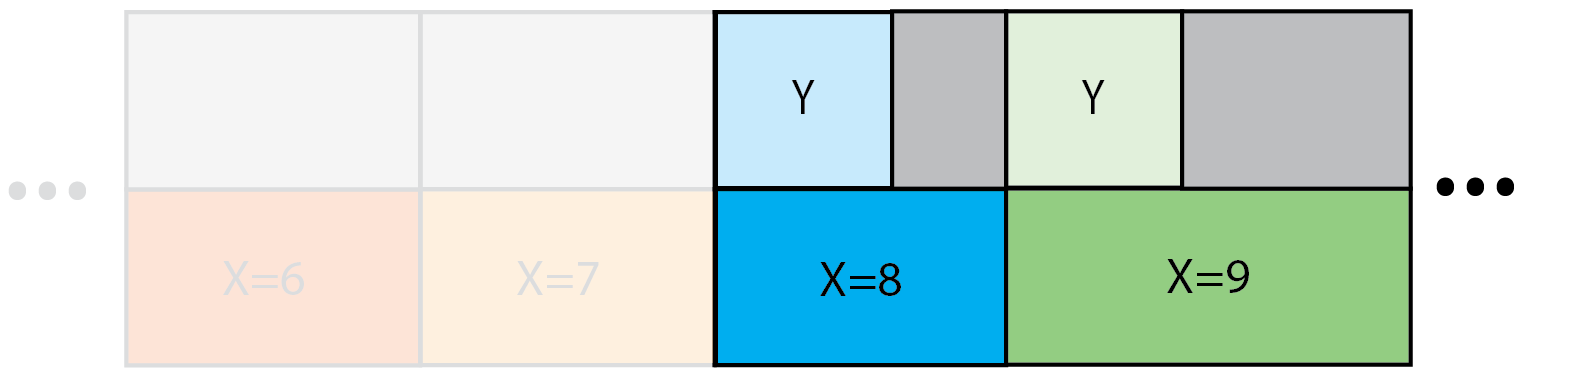
\includegraphics[width=0.8\linewidth]{images/missing-diagram3.png}
	\end{center}
\end{frame}

\begin{frame}{Option 2. Extrapolate}
	Fit a parametric model
	$$ E[Y \mid X \ge 8, R=1] = \beta_0 + \beta_1 X $$
	then fill in missing SBP with model predictions
	\begin{center}
		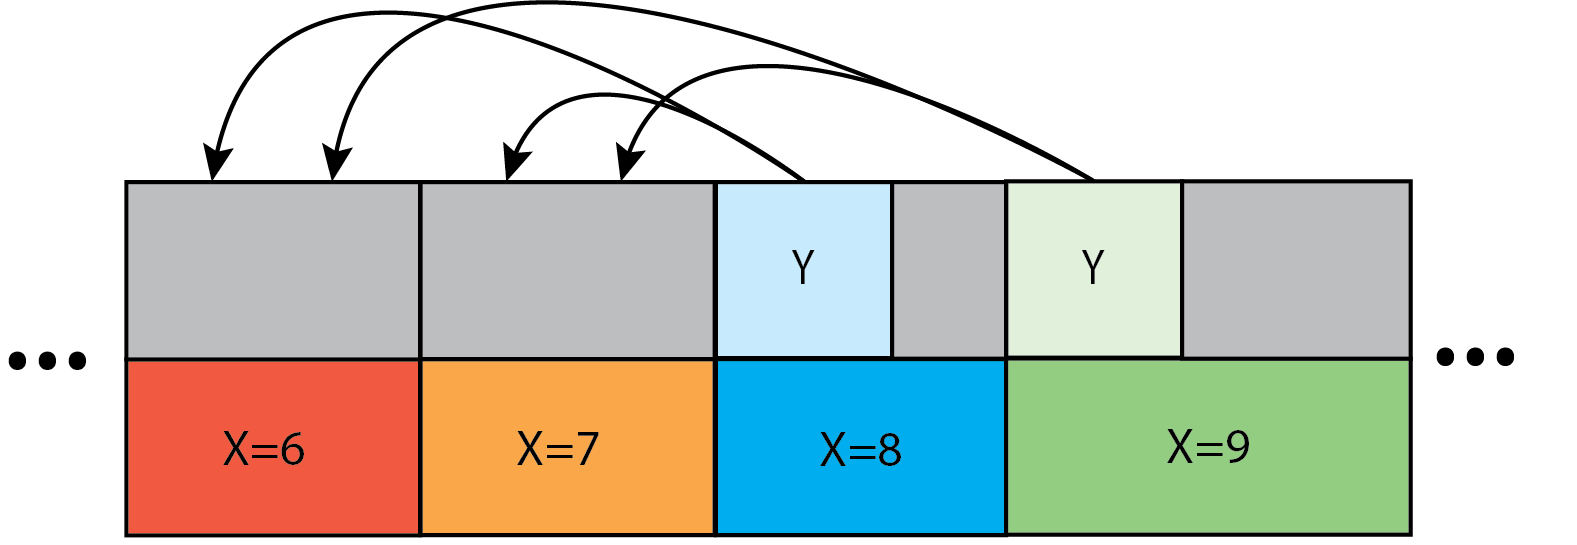
\includegraphics[width=0.7\linewidth]{images/missing-diagram4.png}
	\end{center}
\end{frame}

\begin{frame}{Extrapolation for NHANES}
	\begin{center}
		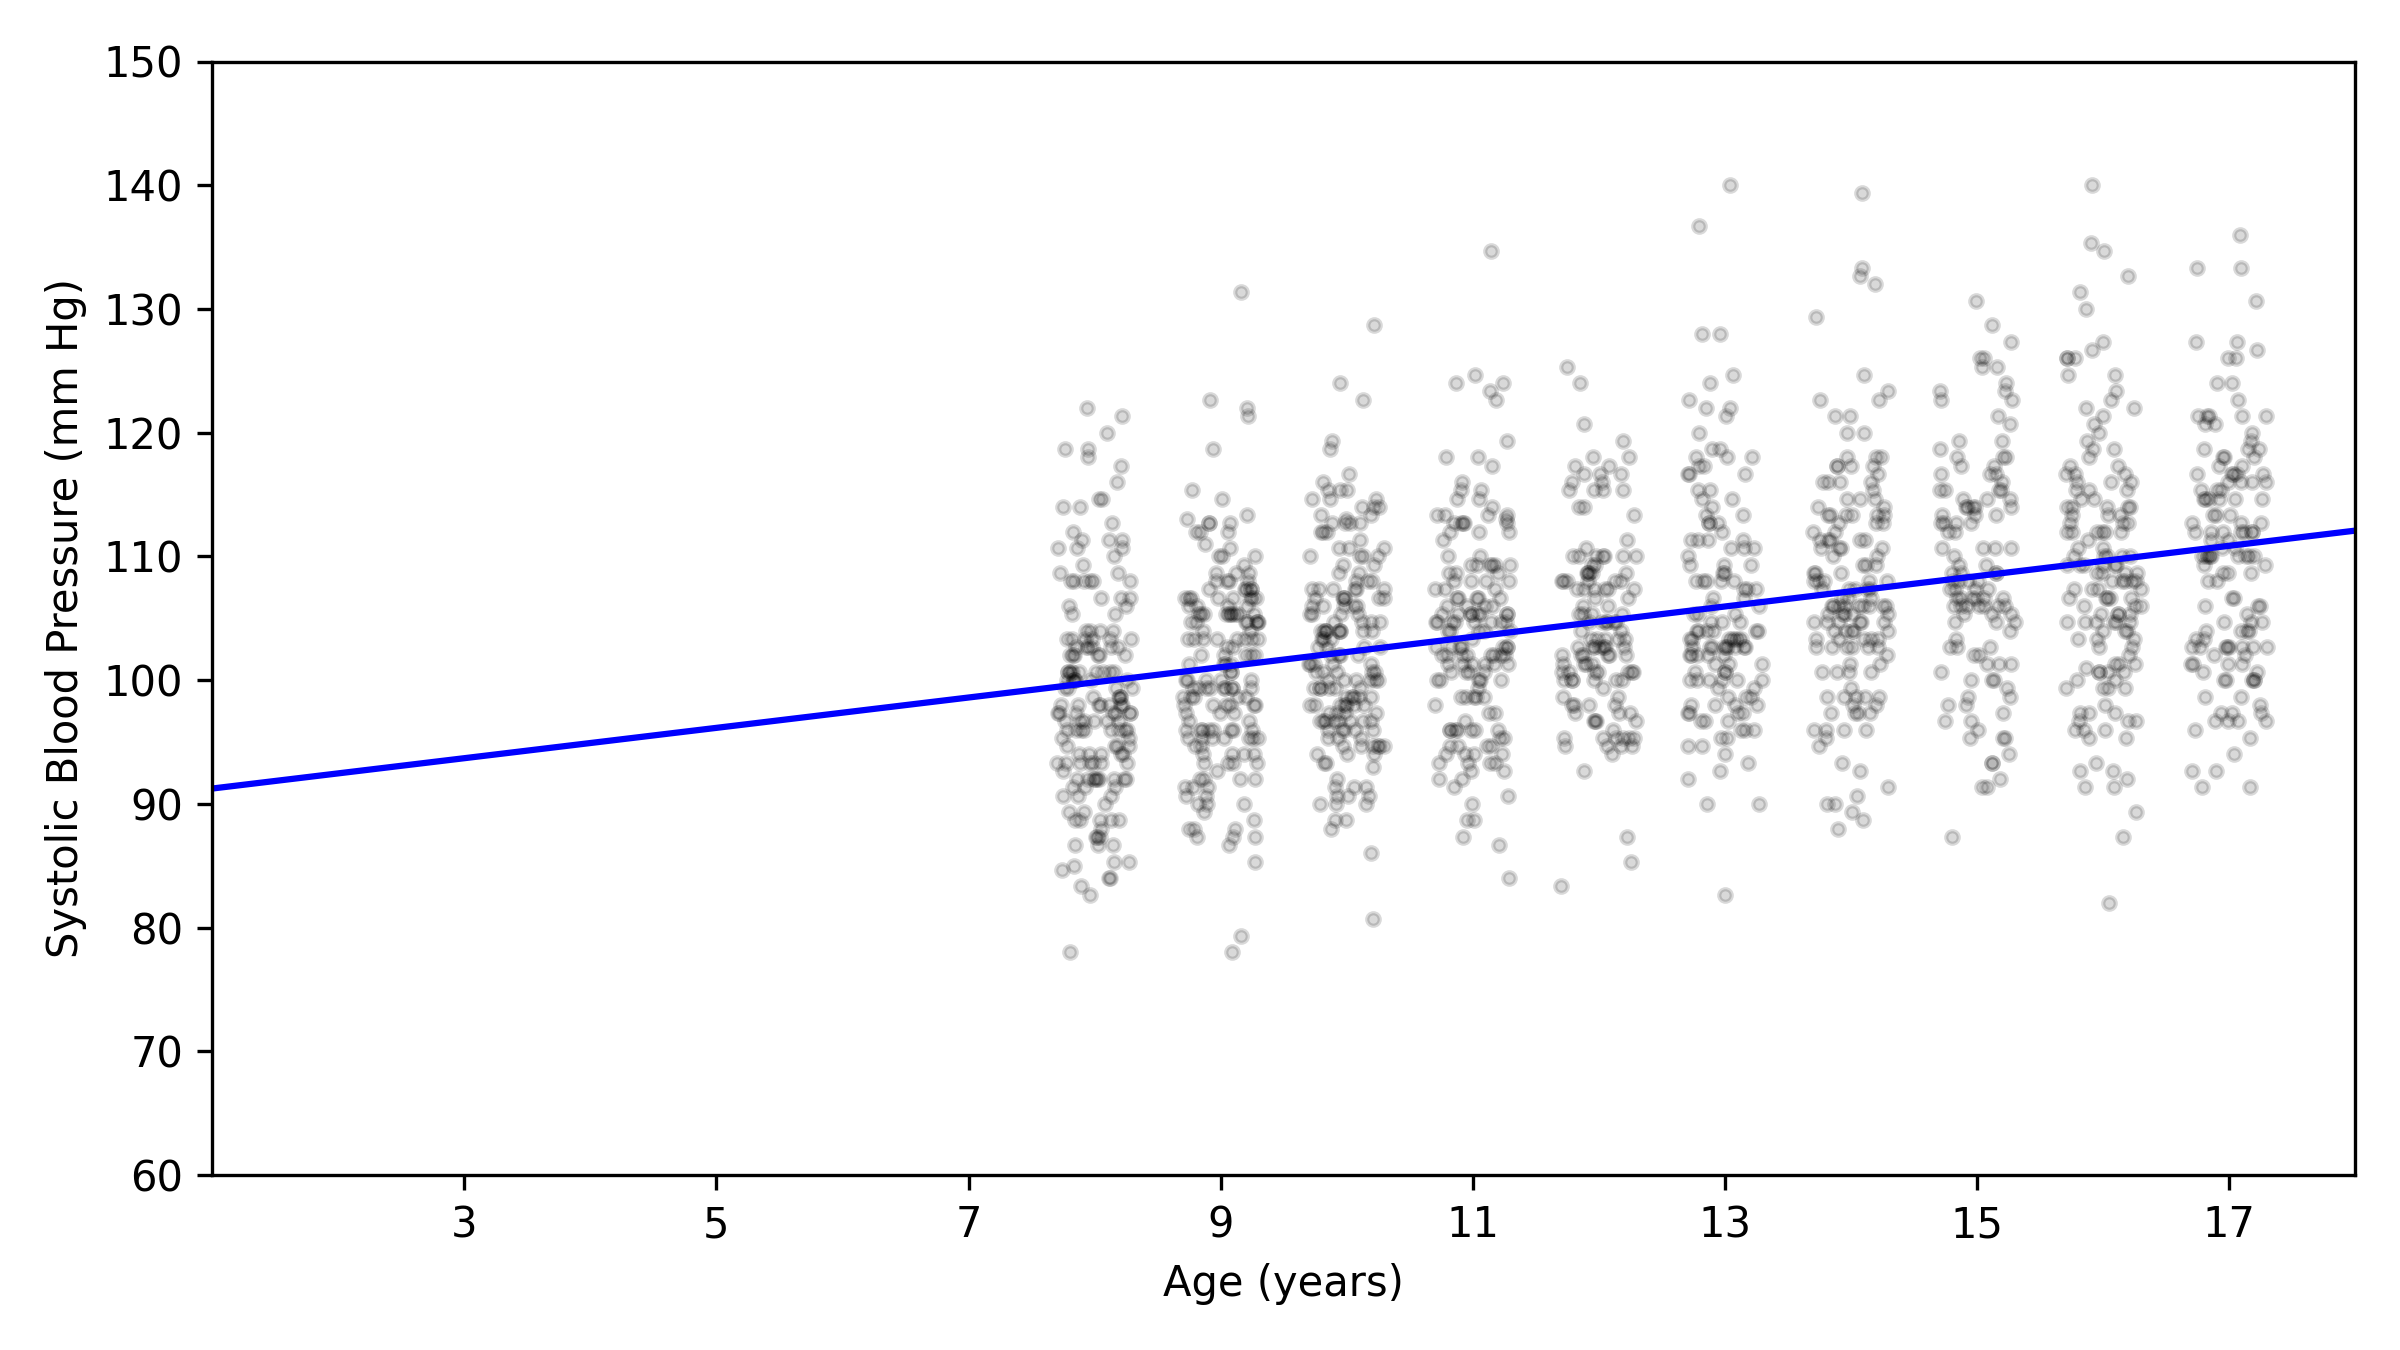
\includegraphics[width=0.92\linewidth]{images/missing_nhanes3.png}
	\end{center}
\end{frame}

\begin{frame}{The Issue with Extrapolation}
	\begin{center}
		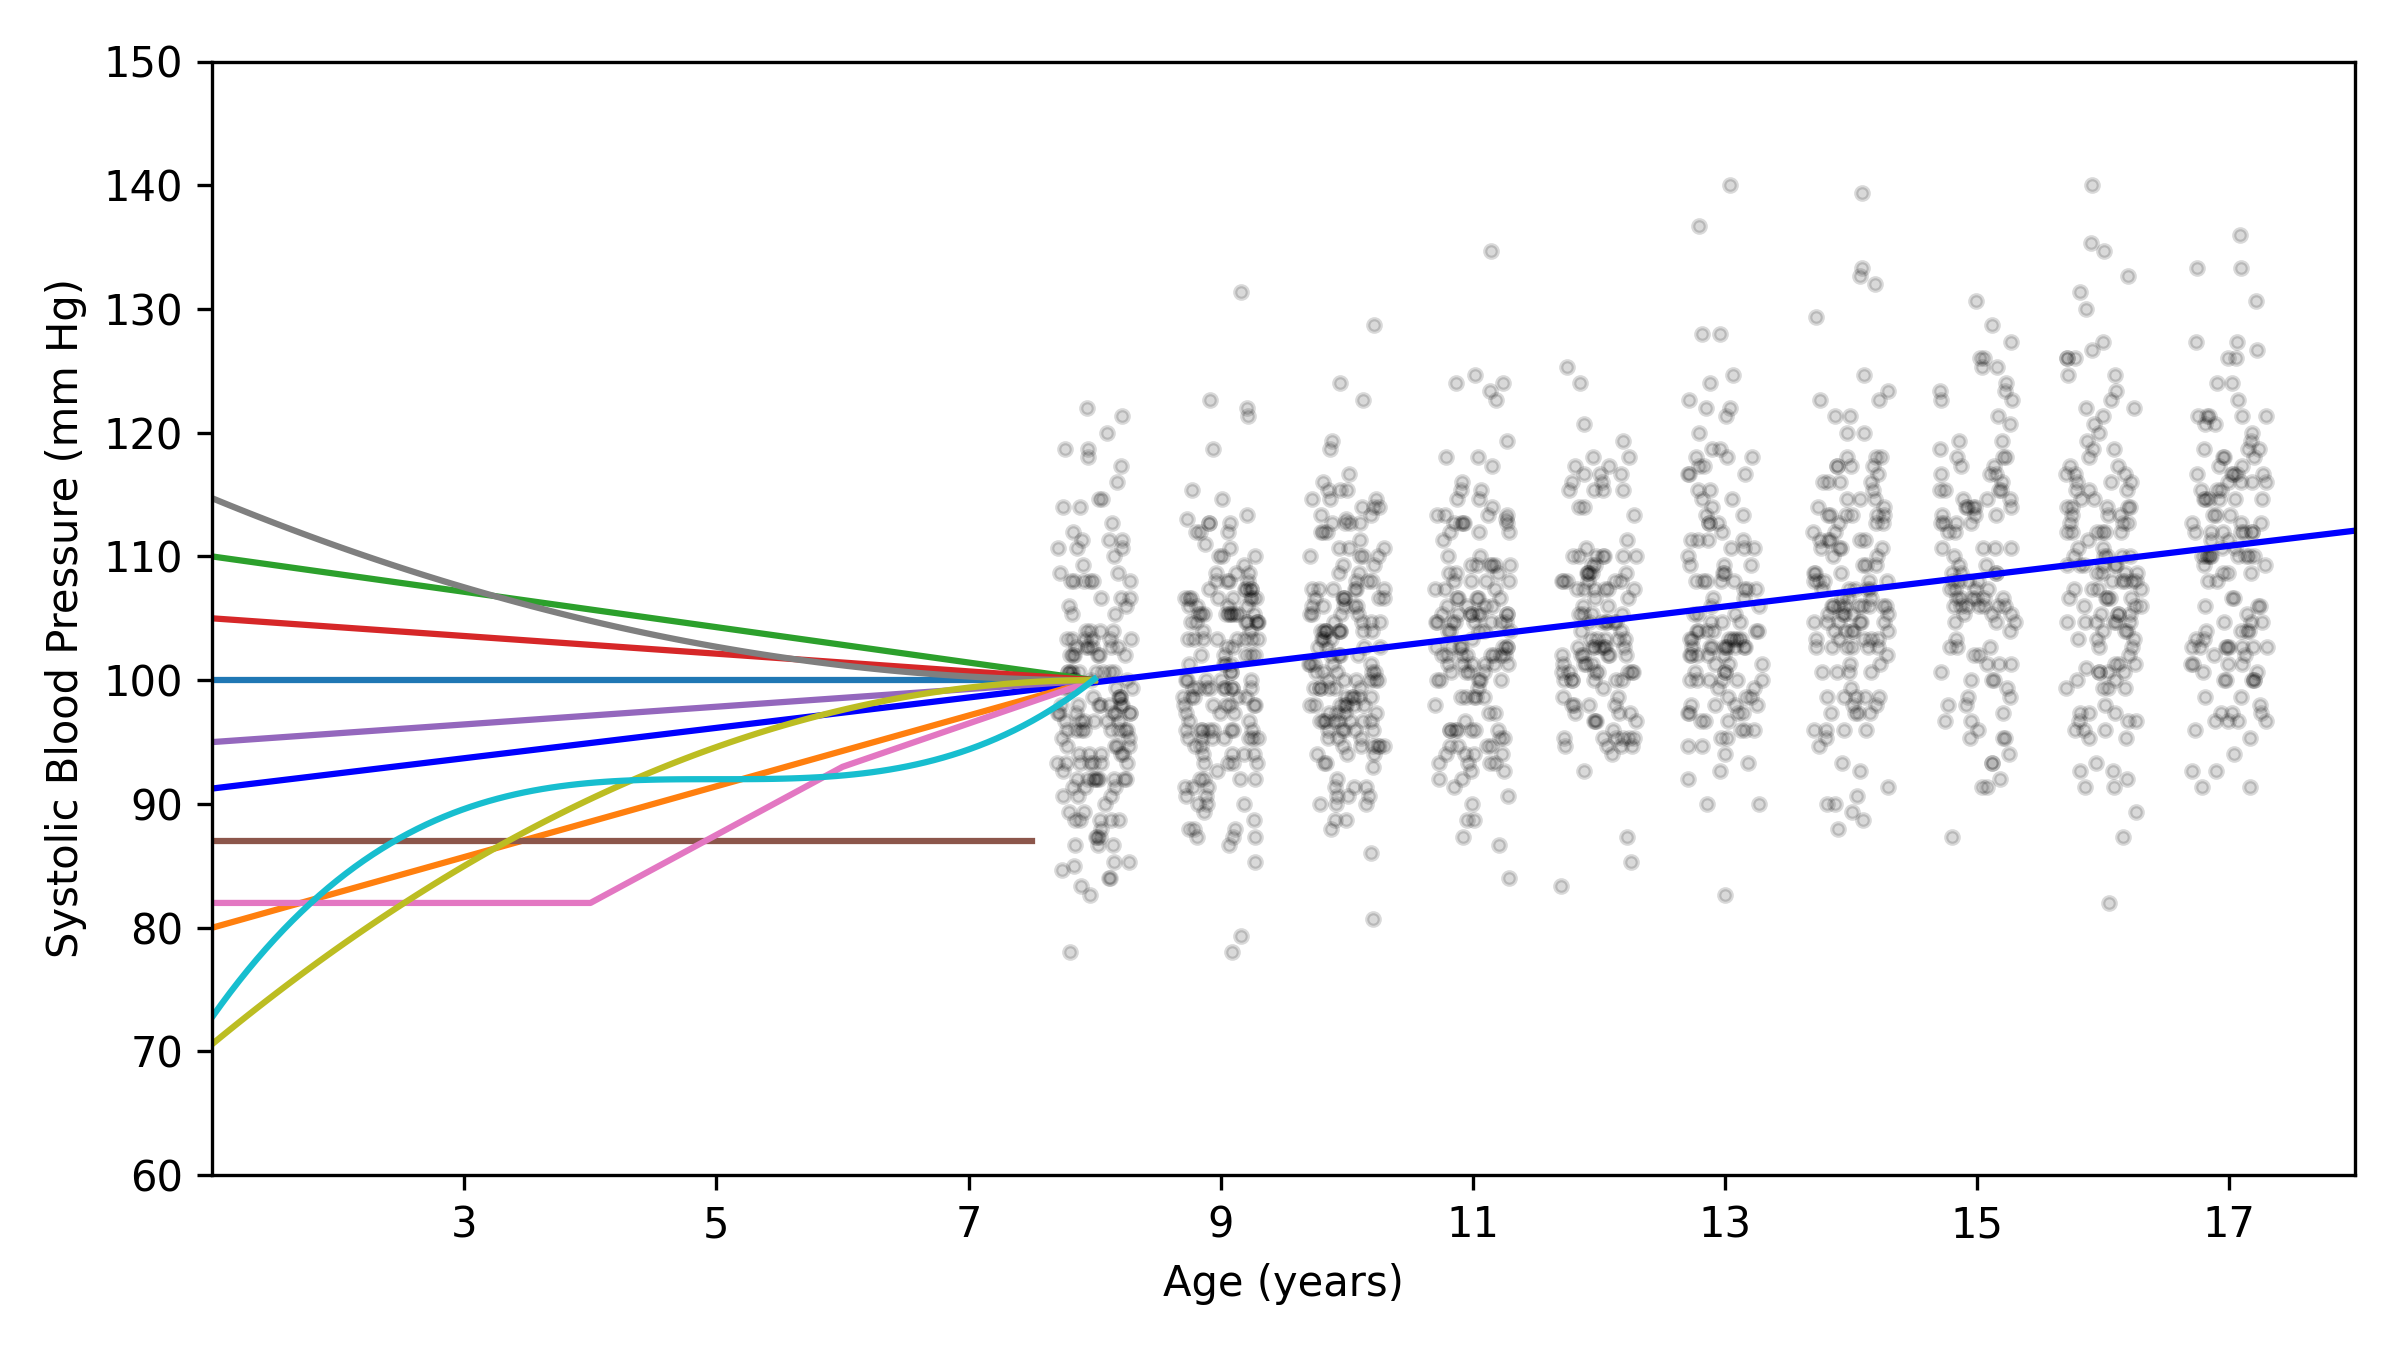
\includegraphics[width=0.92\linewidth]{images/missing_nhanes3b.png}
	\end{center}
\end{frame}

\begin{frame}{An Alternative Approach}
	Divide parameter of interest in parts
	\\~\\
	\begin{equation*}
		\eqnmarkbox[darkgreen]{node0}{\mu} = \eqnmarkbox[blue]{node1}{E[Y \mid X \ge 8]} \Pr(X \ge 8) + \eqnmarkbox[red]{node2}{E[Y \mid X < 8]} \Pr(X < 8)
	\end{equation*}
	\annotate[yshift=0.75em]{above,right}{node0}{Overall mean}	
	\annotate[yshift=-0.4em]{below,right}{node1}{Mean in positive region}	
	\annotate[yshift=0.75em]{above,left}{node2}{Mean in nonpositive region}	
	~\\~\\
	\textbf{Strategy}: divide and conquer
	~\\~\\
	Here, we can still identify the mean in the positive region
	$$ \mu^* = \eqnmarkbox[blue]{nodeZ}{E[Y \mid X \ge 8]} = \sum_{x \in \mathcal{X}} E(Y \mid R=1, X=x, X \ge 8) \Pr(X=x \mid X \ge 8) $$
\end{frame}

\begin{frame}{Dealing with Non-Positivity}
	Available data leaves us stuck with $ \eqnmarkbox[red]{nodeZ}{E[Y \mid X < 8]} = \; ?$
	\begin{itemize}
		\item To progress, will appeal to external information
	\end{itemize}
	~\\
	\begin{center}
		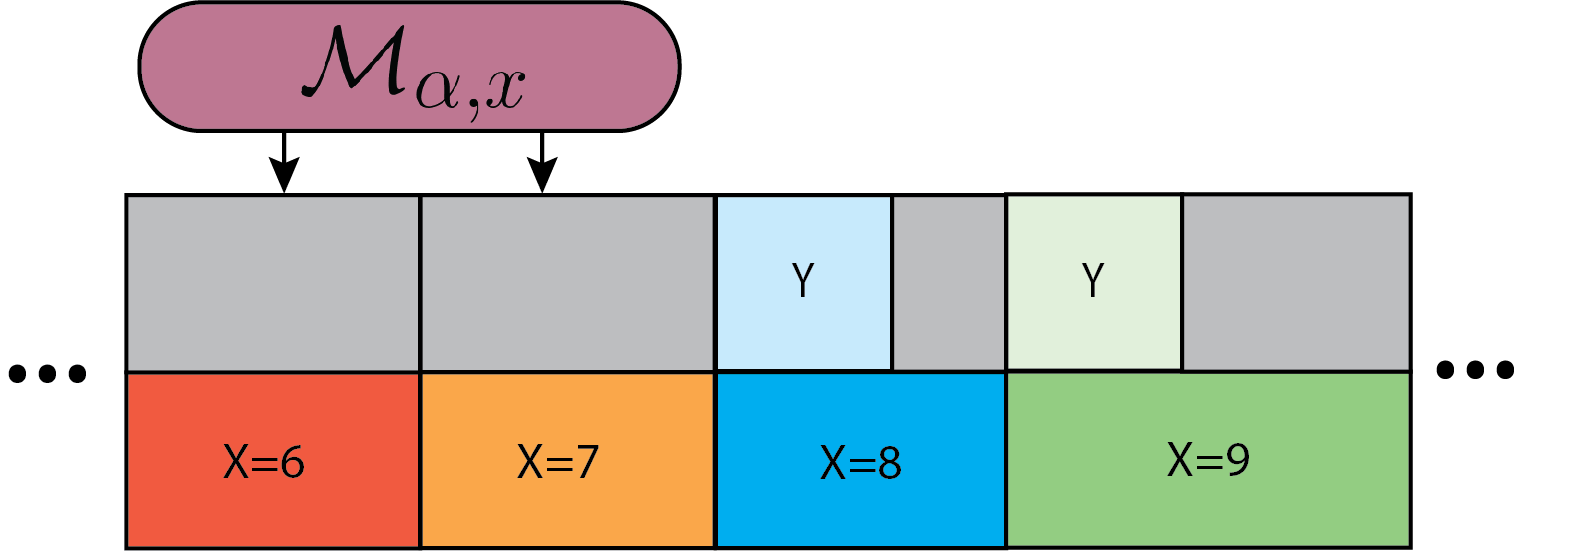
\includegraphics[width=0.8\linewidth]{images/missing-diagram5.png}
	\end{center}
\end{frame}

\begin{frame}{Constructing Bounds}
	At the most basic level, we know that SBP must be a (finite) positive number
	$$ E[Y \mid X=x] \in (0, c) \text{ where } c<\infty \text{ for ages 2-7}$$
	~\\
	Context allows us to further narrow the plausible region to
	$$ E[Y \mid X=x] \in [50, 140] \text{ for ages 2-7}$$
	as these boundary values would constitute medical emergencies
\end{frame}

\begin{frame}{Constructing Bounds}
	Following some algebra, we can show that $\mu$ must be greater than
	$$ 50 + \Pr(X \ge 8)\left\{\eqnmarkbox[blue]{nodeZ1}{E[Y \mid X \ge 8]} - 50\right\}$$  
	and less than
	$$140 + \Pr(X \ge 8)\left\{\eqnmarkbox[blue]{nodeZ2}{E[Y \mid X \ge 8]} - 140\right\}$$ 
\end{frame}

\begin{frame}{Sensitivity Analysis}
	In this example, the bounds are quite wide, $[85.8, 116.8]$
	~\\~\\~\\
	Rather than evaluate at the extremes, evaluate
	\begin{equation*}
		\eqnmarkbox[darkgreen]{node0}{\mu} = \eqnmarkbox[blue]{node1}{ \sum_{x \in \mathcal{X}} E(Y \mid R=1, X=x, X \ge 8) \Pr(X=x \mid X \ge 8)} \Pr(X \ge 8) + \eqnmarkbox[red]{node2}{q} \Pr(X < 8)
	\end{equation*}
	where $q$ is set to a particular value
	~\\~\\~\\
	Some readers might be more optimistic than others
	\begin{itemize}
		\item Rather than select one $q$ for everyone, can show how $\mu$ varies as a function of $q$
	\end{itemize}
\end{frame}

\begin{frame}{Sensitivity Analysis Estimator}
	Our algebra before gave us the following formula
	\begin{equation*}
		\eqnmarkbox[red]{nodeZ2}{q} + \Pr(X \ge 8)\left\{\eqnmarkbox[blue]{nodeZ1}{E[Y \mid X \ge 8]} - \eqnmarkbox[red]{nodeZ3}{q}\right\}
	\end{equation*}
	~\\
	I will use g-computation to estimate $\eqnmarkbox[blue]{nodeZ1}{E[Y \mid X \ge 8]}$,\footnote[frame]{Cole et al. \textit{Am J Epidemiol}, 2023; 192(1):6-10} but could use IPW or AIPW
	~\\~\\~\\
	95\% Confidence intervals are computed using the sandwich variance with $q$ held fixed\footnote[frame]{Ross et al. \textit{Int J Epidemiol} 2024; 53(2):dyae030}
\end{frame}

\begin{frame}{Results by Method}
	\begin{center}
		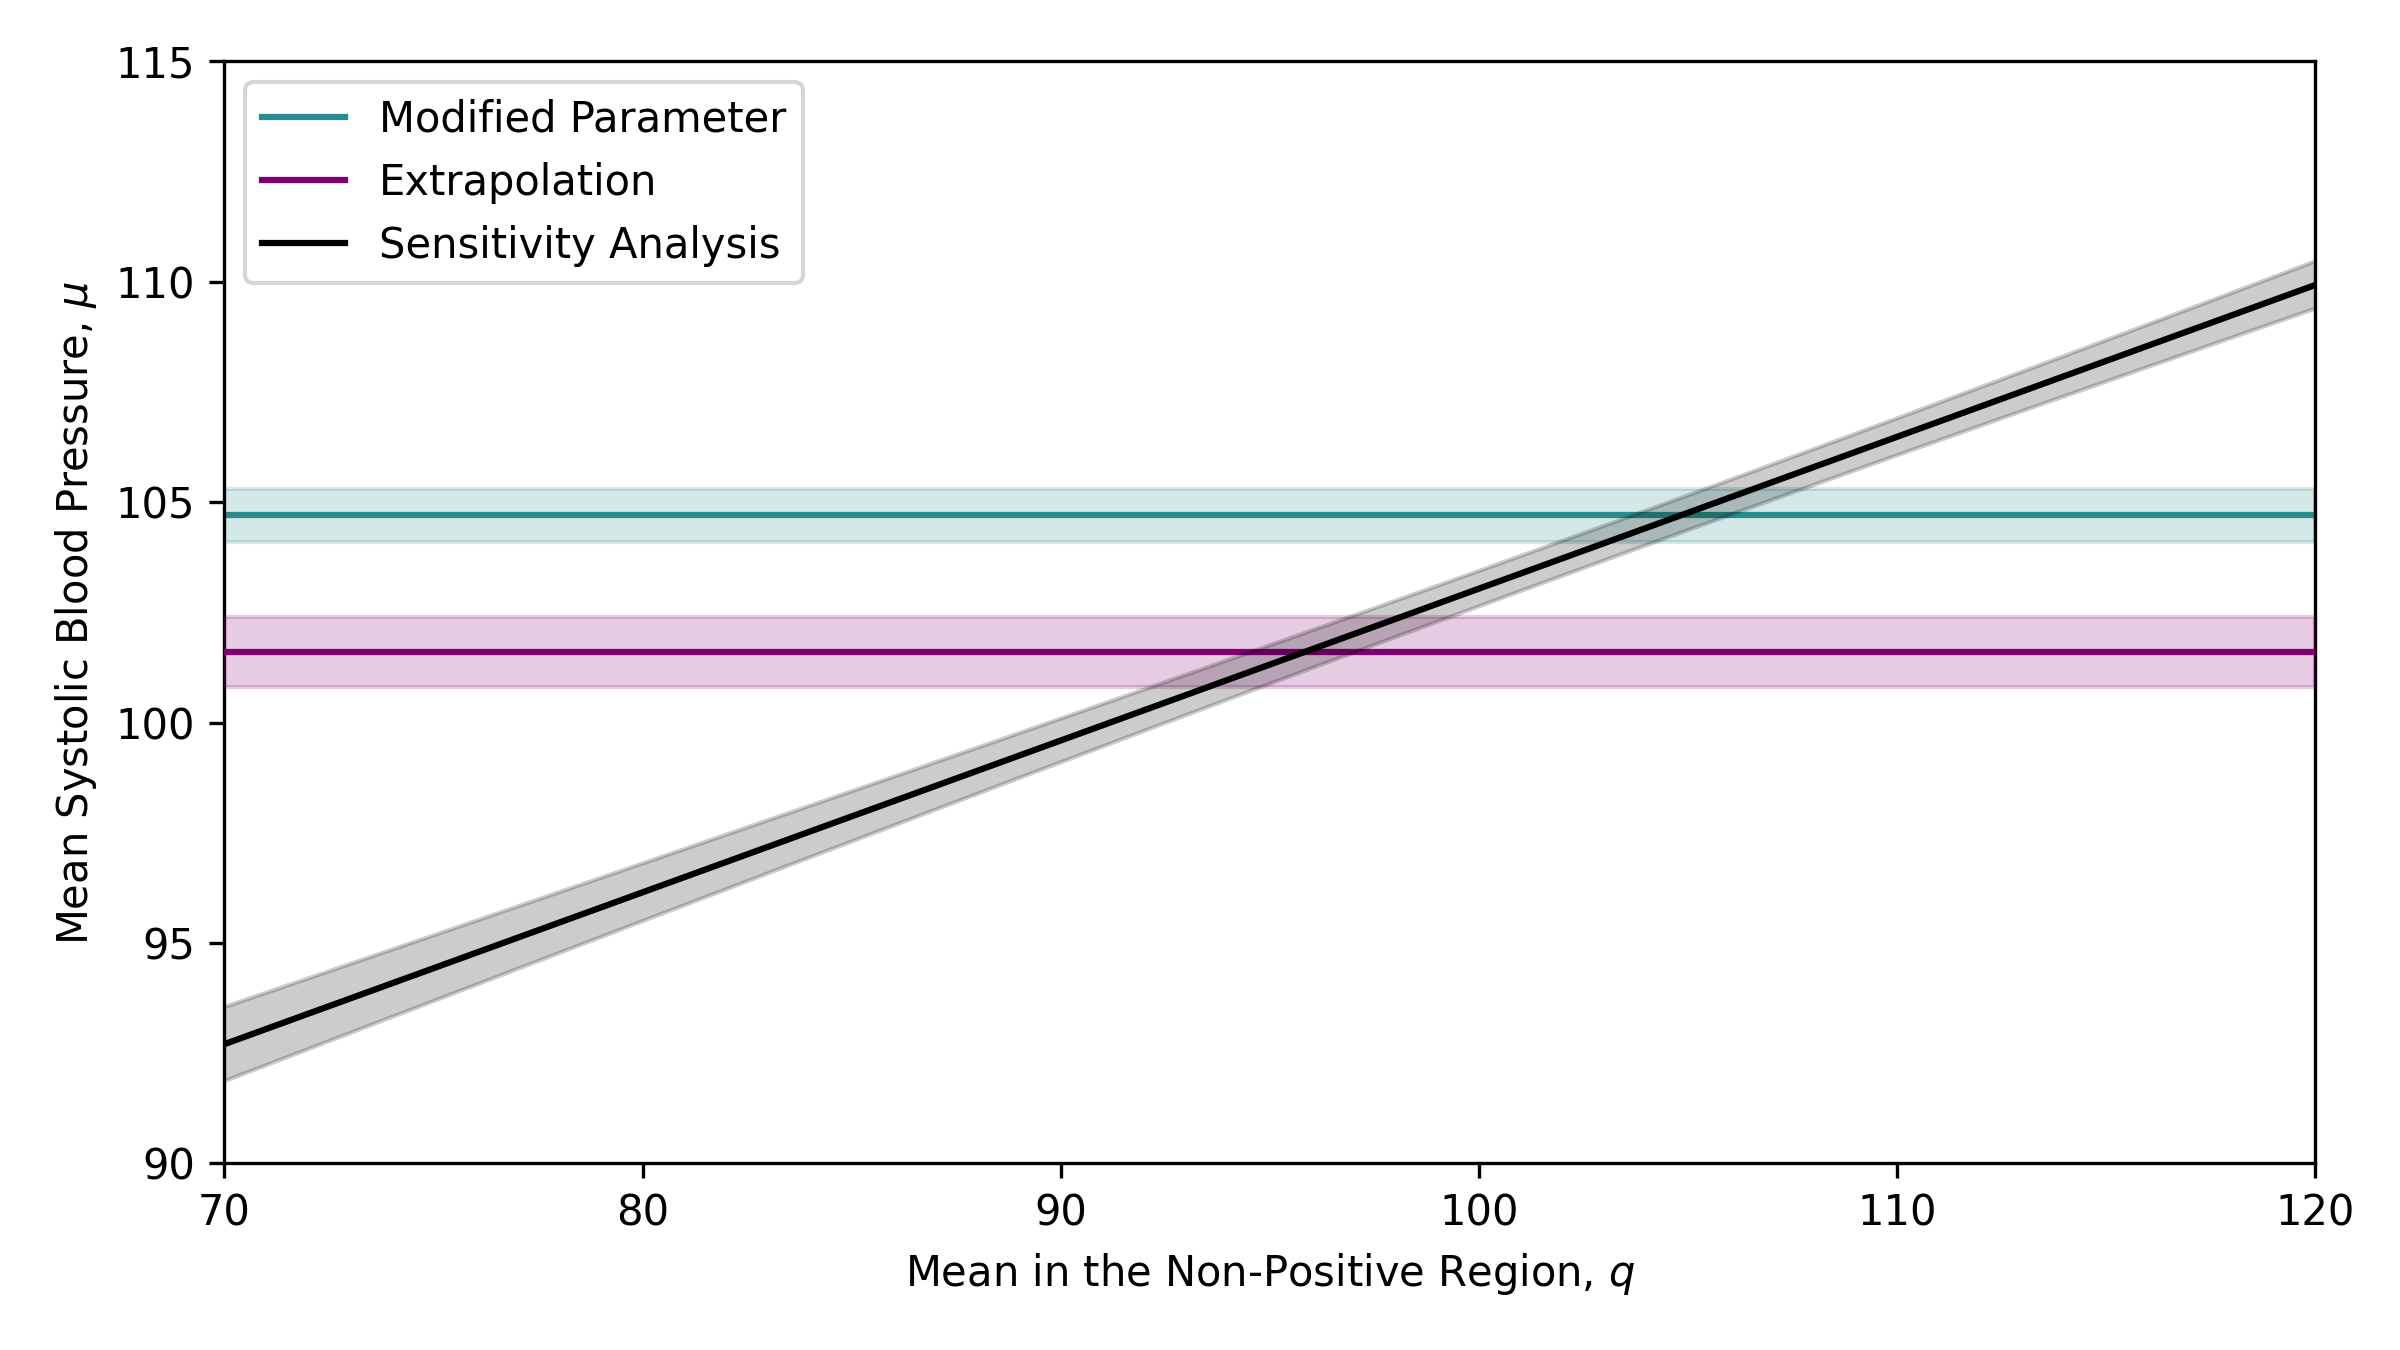
\includegraphics[width=0.92\linewidth]{images/missing_sens_results.png}
	\end{center}
\end{frame}

\section{Conclusions}

\begin{frame}{Summary}	
	Positivity is often neglected as an assumption
	\begin{itemize}
		\item But it remains vital for identification of many parameters
	\end{itemize}
	~\\
	Restricting parameters to positive regions may be reasonable
	\begin{itemize}
		\item But may limit utility of research
		\item Extrapolation premised on strong assumptions
	\end{itemize}
	~\\
	Approach described here (1) retain interest parameter, and (2) less strict assumptions
\end{frame}

\begin{frame}{Extensions}	
	Replace fixed $q$ with a distribution
	\begin{itemize}
		\item Can further replace $q$ with a mathematical model to incorporate more rich external information\footnote[frame]{Some work on formalizing identification with mathematical models: Zivich \textit{arXiv:2511.01960}}
	\end{itemize}
	~\\
	Exchangeability (and thus positivity) is used to address other systematic errors
	\begin{itemize}
		\item Approach can be used to address nonpositivity in these settings\footnote[frame]{Originally proposed in the context of transporting trials: Zivich et al. \textit{Epidemiology} 2024;35(1):23-31, Zivich et al. \textit{JRSSA} 2025;188(1):158-180}
	\end{itemize}
	~\\
	Approach based on knowledge of the $X$ where non-positivity occurs\footnote[frame]{Susmann et al. \textit{arXiv:2509.20206} have an approach based on the propensity score that does not require this knowledge to construct corresponding bounds}
\end{frame}

\begin{frame}{Thank You!}
	\textbf{Publication}: Zivich et al. \textit{J Epidemiol Community Health} 2026;80:352-356
	~\\~\\~\\~\\
	\begin{center}
		\small
		\faEnvelope \quad pzivich@unc.edu \qquad \quad 
		\faGithub \quad pzivich \qquad \quad
		\faHashtag \quad pausalz@bsky.social
	\end{center}	
\end{frame}

\section{Appendix}

\begin{frame}{Why Positivity Matters}
	Following definition of conditional expectation
	$$ E[Y \mid X=x, R=1] = \frac{E[Y R \; I(X=x)]}{\Pr(R=1 \mid X=x) \Pr(X=x)}$$
	~\\
	So $\Pr(R=1 \mid X=x)$ results in a division by zero when positivity is not met
\end{frame}

\begin{frame}{Synthesis of Statistical and Mathematical Models}
	\begin{center}
		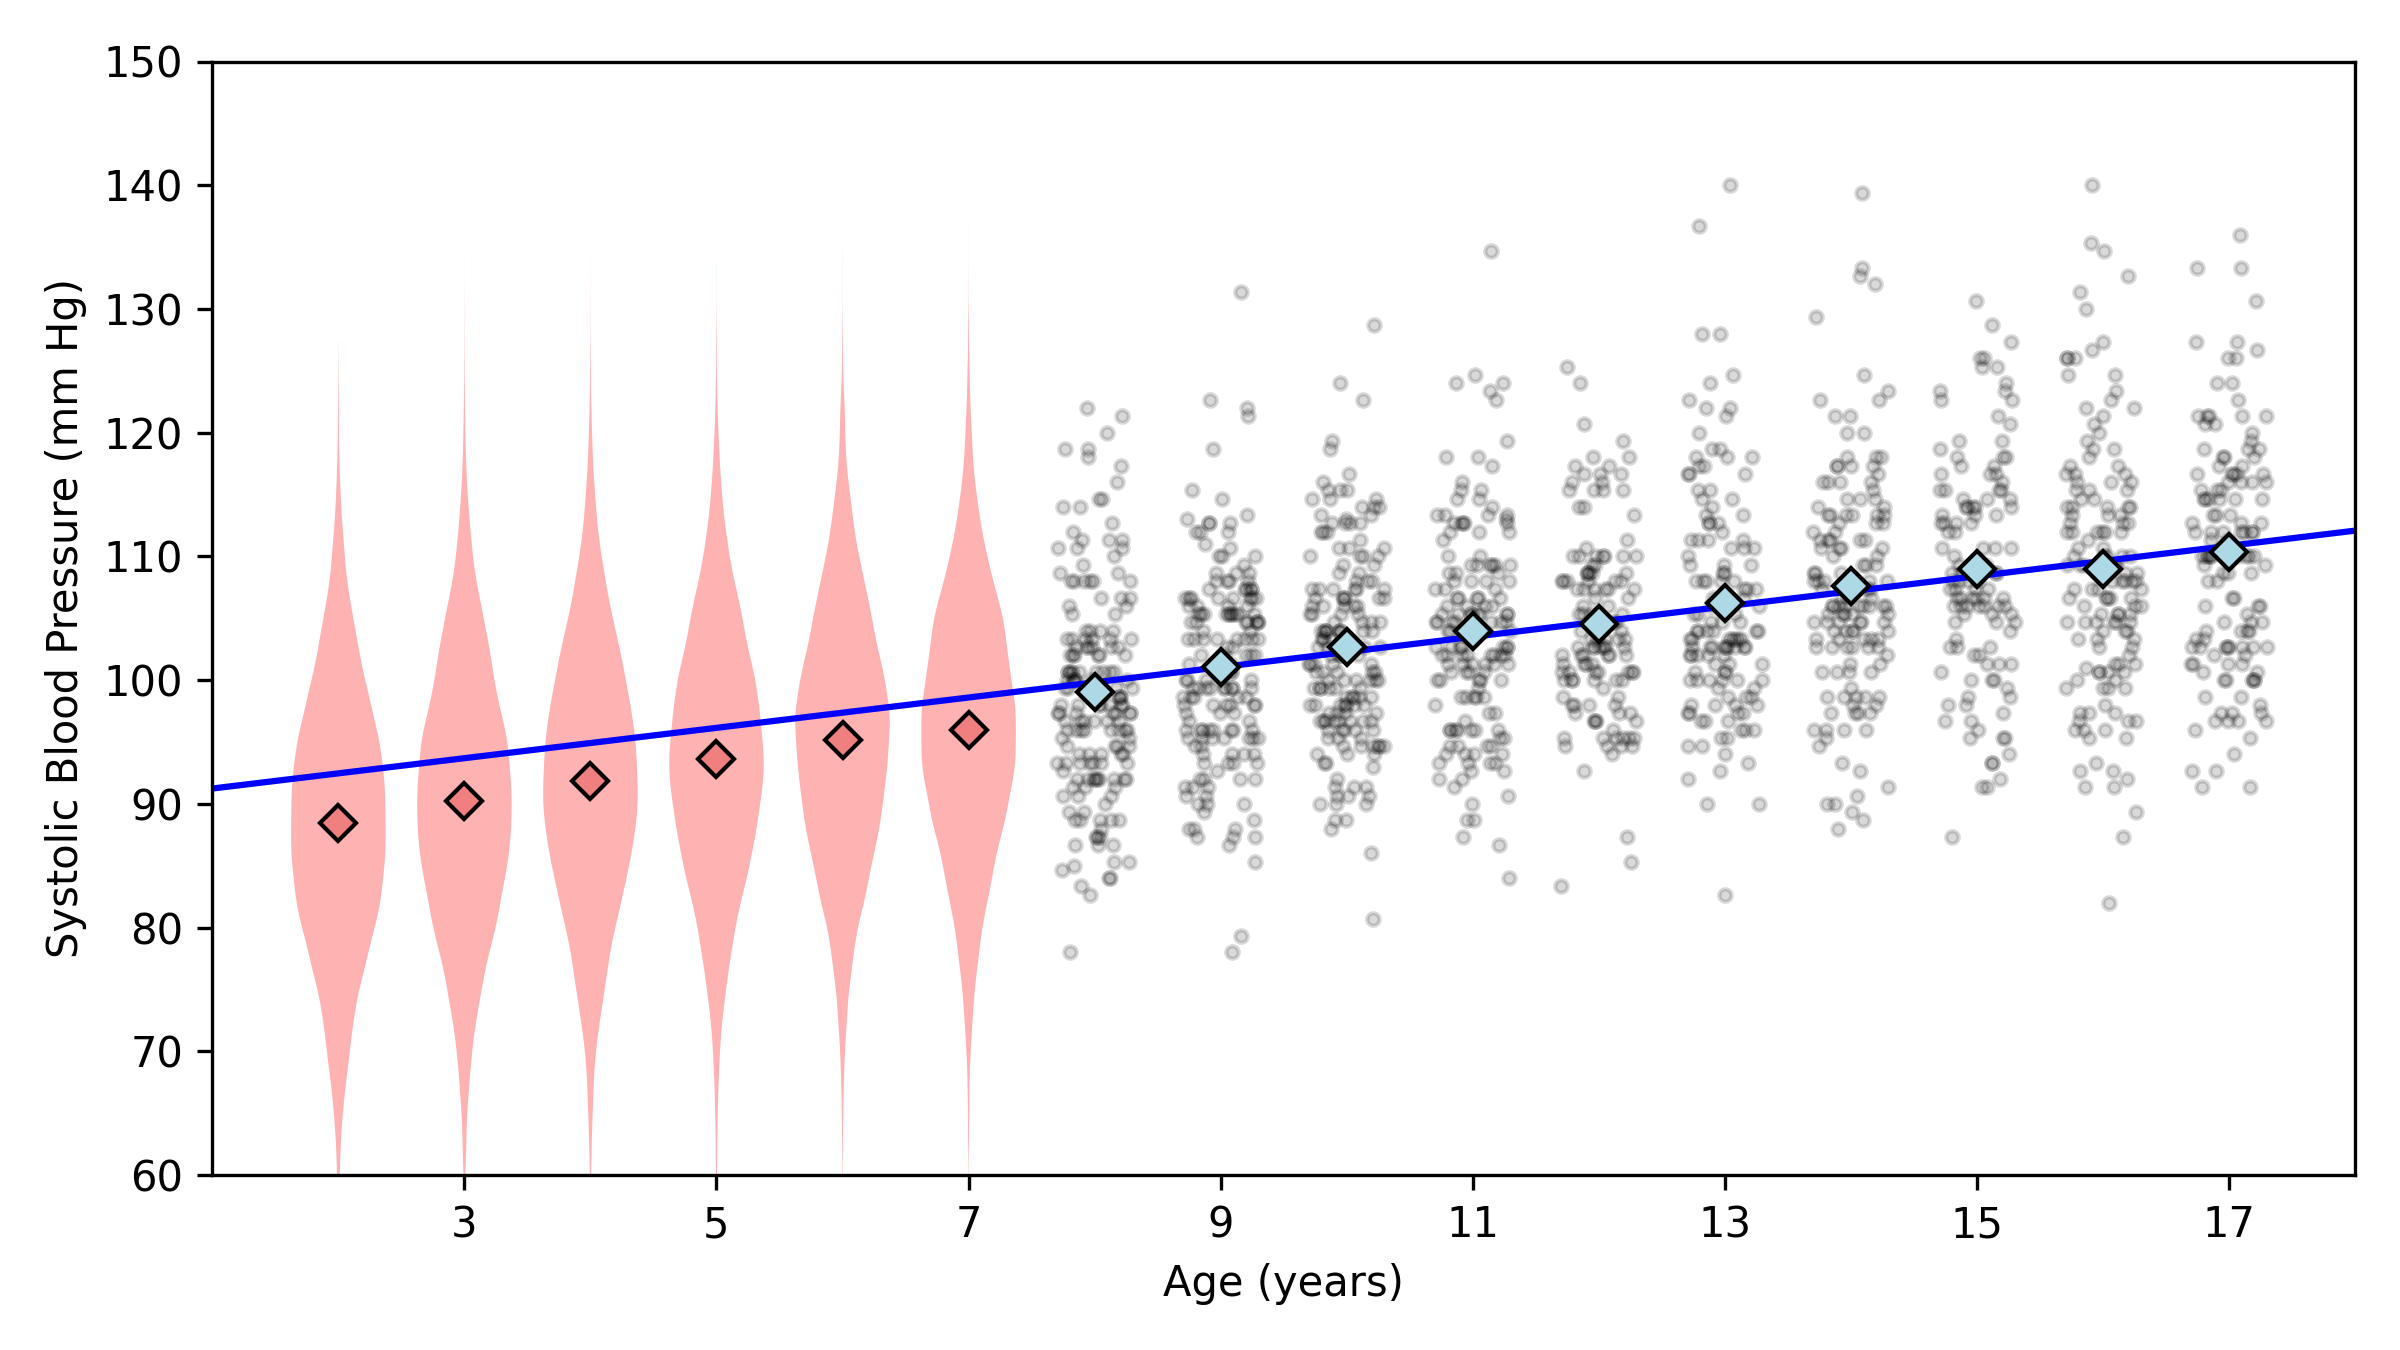
\includegraphics[width=0.85\linewidth]{images/missing_nhanes4.png}
	\end{center}
\end{frame}

\end{document}